\chapter{Nucleoside and nucleobase quantification}



\begin{figure}[!ht]
     \centering
     \begin{subfigure}[b]{0.68\textwidth}
         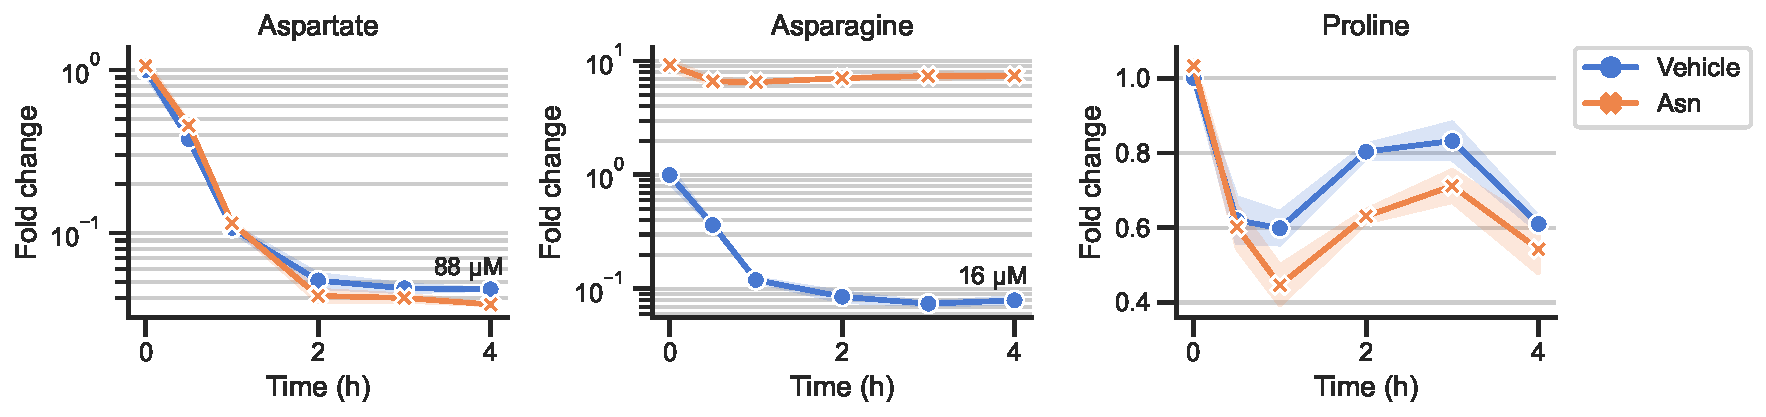
\includegraphics[width=\textwidth]{figures/chap2/app/HT1080_Anti_AA.pdf}
         \caption{Amino acids}
         \label{fig:app_ch2:HT1080_Anti_AA}
     \end{subfigure}
     \hfill
     \begin{subfigure}[b]{0.45\textwidth}
         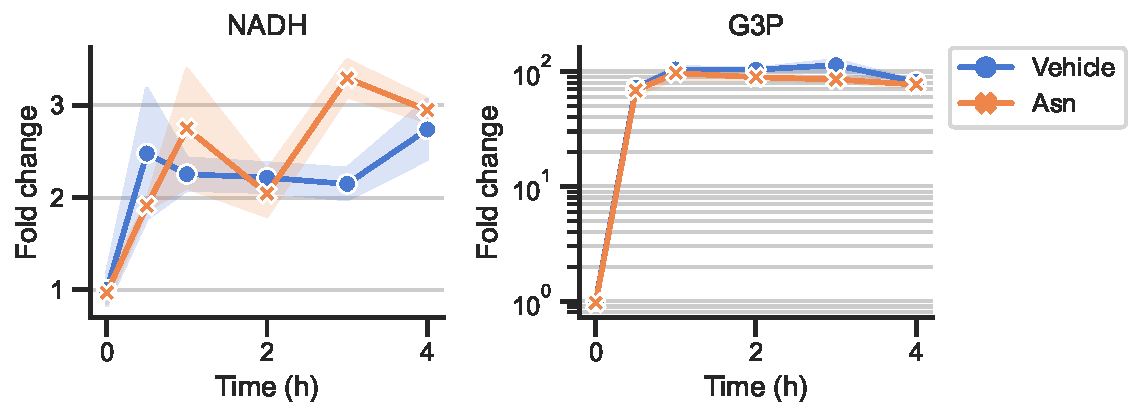
\includegraphics[width=\textwidth]{figures/chap2/app/HT1080_Anti_rd.pdf}
         \caption{Redox metabolites}
         \label{fig:app_ch2:HT1080_Anti_rd}
     \end{subfigure}
     \hfill
     \begin{subfigure}[b]{0.9\textwidth}
         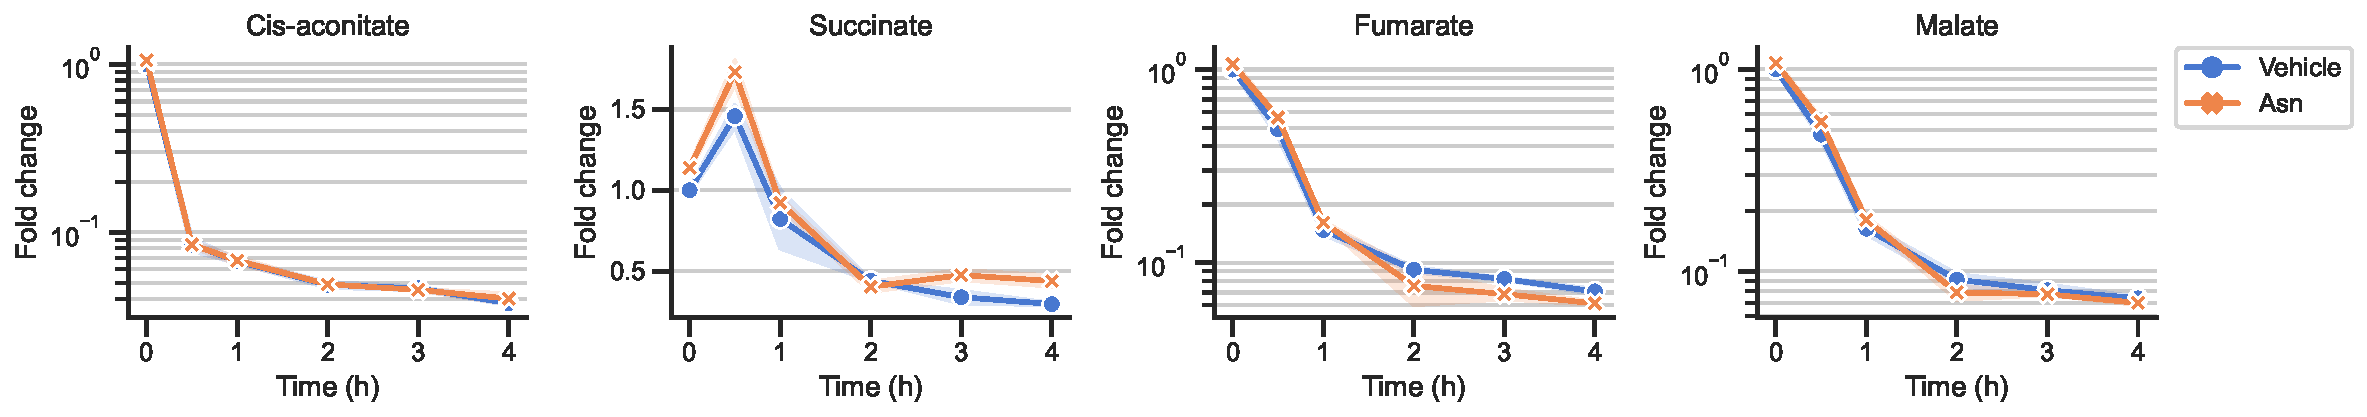
\includegraphics[width=\textwidth]{figures/chap2/app/HT1080_Anti_tca.pdf}
         \caption{TCA metabolites}
         \label{fig:app_ch2:HT1080_Anti_tca}
     \end{subfigure}
     \hfill
     \begin{subfigure}[b]{0.9\textwidth}
         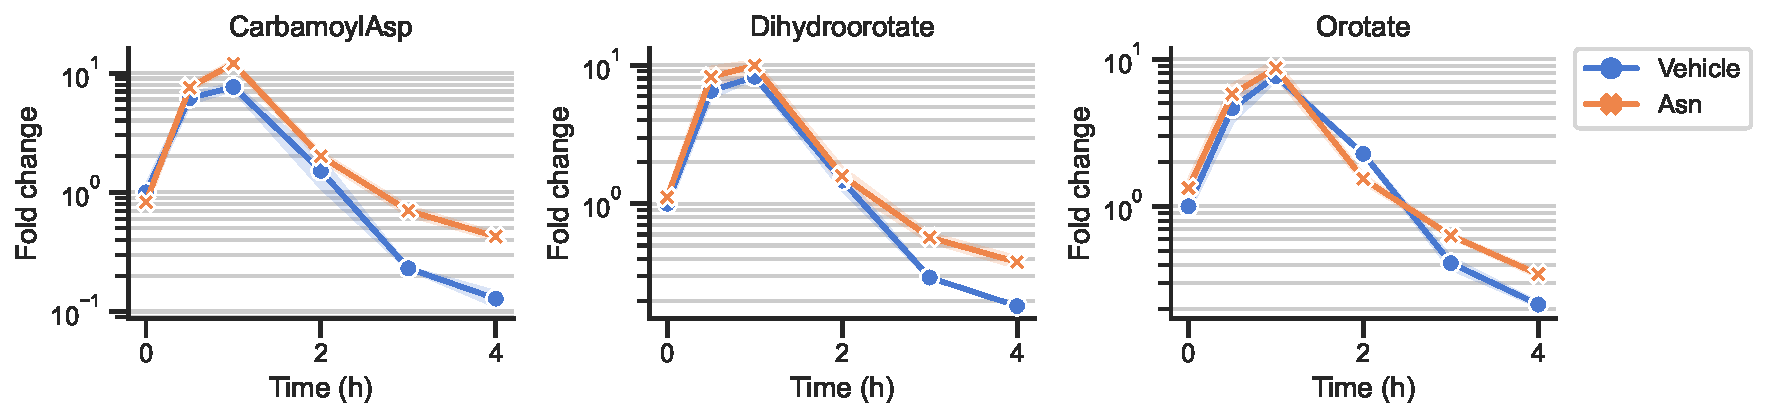
\includegraphics[width=\textwidth]{figures/chap2/app/HT1080_Anti_pyr.pdf}
         \caption{Pyrimidine metabolites}
         \label{fig:app_ch2:HT1080_Anti_pyr}
     \end{subfigure}
     \hfill
     \begin{subfigure}[b]{0.45\textwidth}
         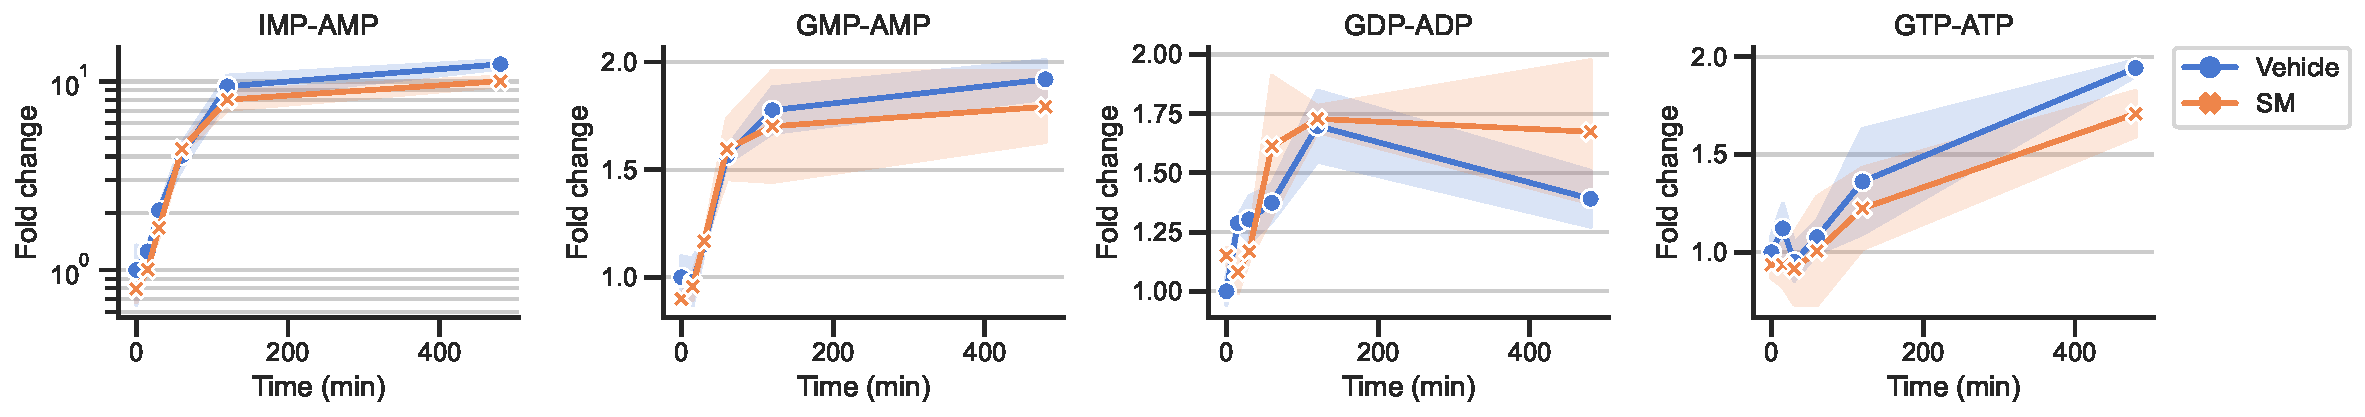
\includegraphics[width=\textwidth]{figures/chap2/app/HT1080_DKO_pur.pdf}
         \caption{Purine metabolites (and dTTP)}
         \label{fig:app_ch2:HT1080_Anti_pur}
     \end{subfigure}
     \hfill
        \caption[Metabolic changes in HT1080 after antimycin treatment]{
        Metabolic changes in HT1080 WT after antimycin (1 µM) treatment.
        From same experiment as figure \ref{fig:ch2:ISR_resc}.
        }
        \label{fig:app_ch2:HT1080_Anti_metab}
\end{figure}



















\begin{figure}
    \centering
    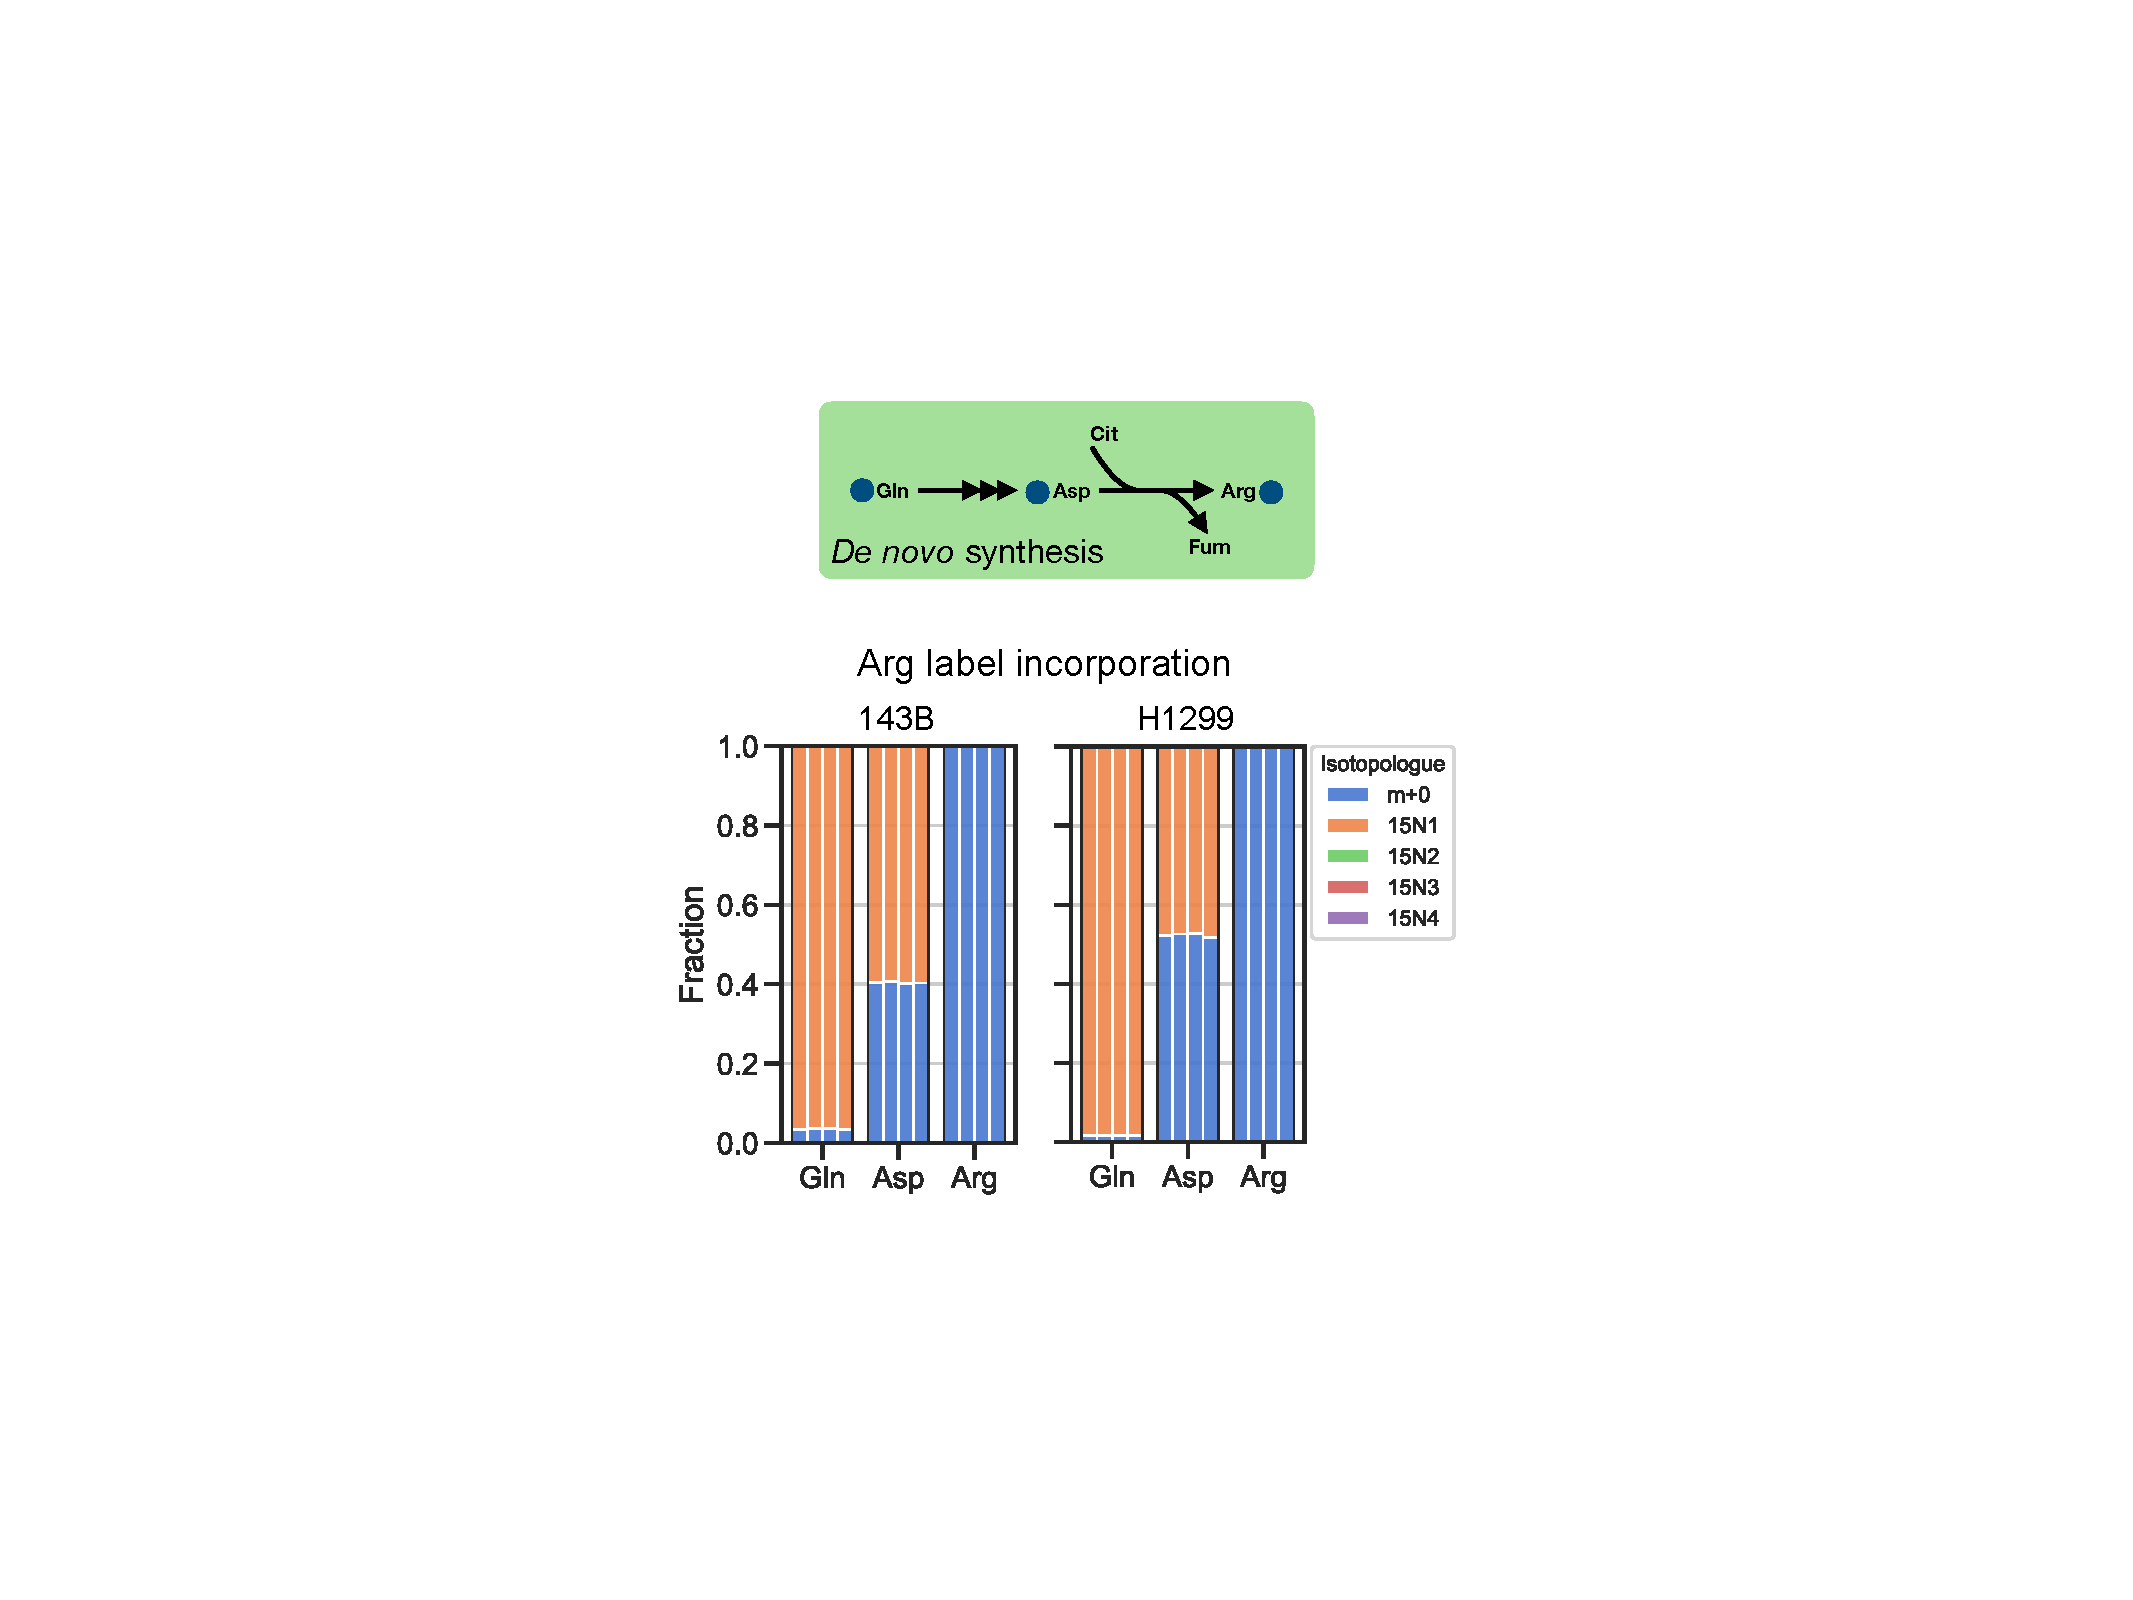
\includegraphics[width=0.45\textwidth]{figures/chap2/app/arg_syn.pdf}
    \caption[No evidence of arginine synthesis in DMEM]{
    No evidence of arginine synthesis in DMEM.
    Top diagram shows Gln alpha\=/\hNi{} label incorporation into Asp and subsequently Arg.
    Bottom isotopologue distribution shows Gln alpha\=/\hNi{} label incorporation into Gln, Asp and Arg at steady-state for cell lines 143B and H1299 grown in DMEM.
    }
    \label{fig:app_ch2:arg_syn}
\end{figure}










\begin{figure}
    \centering
    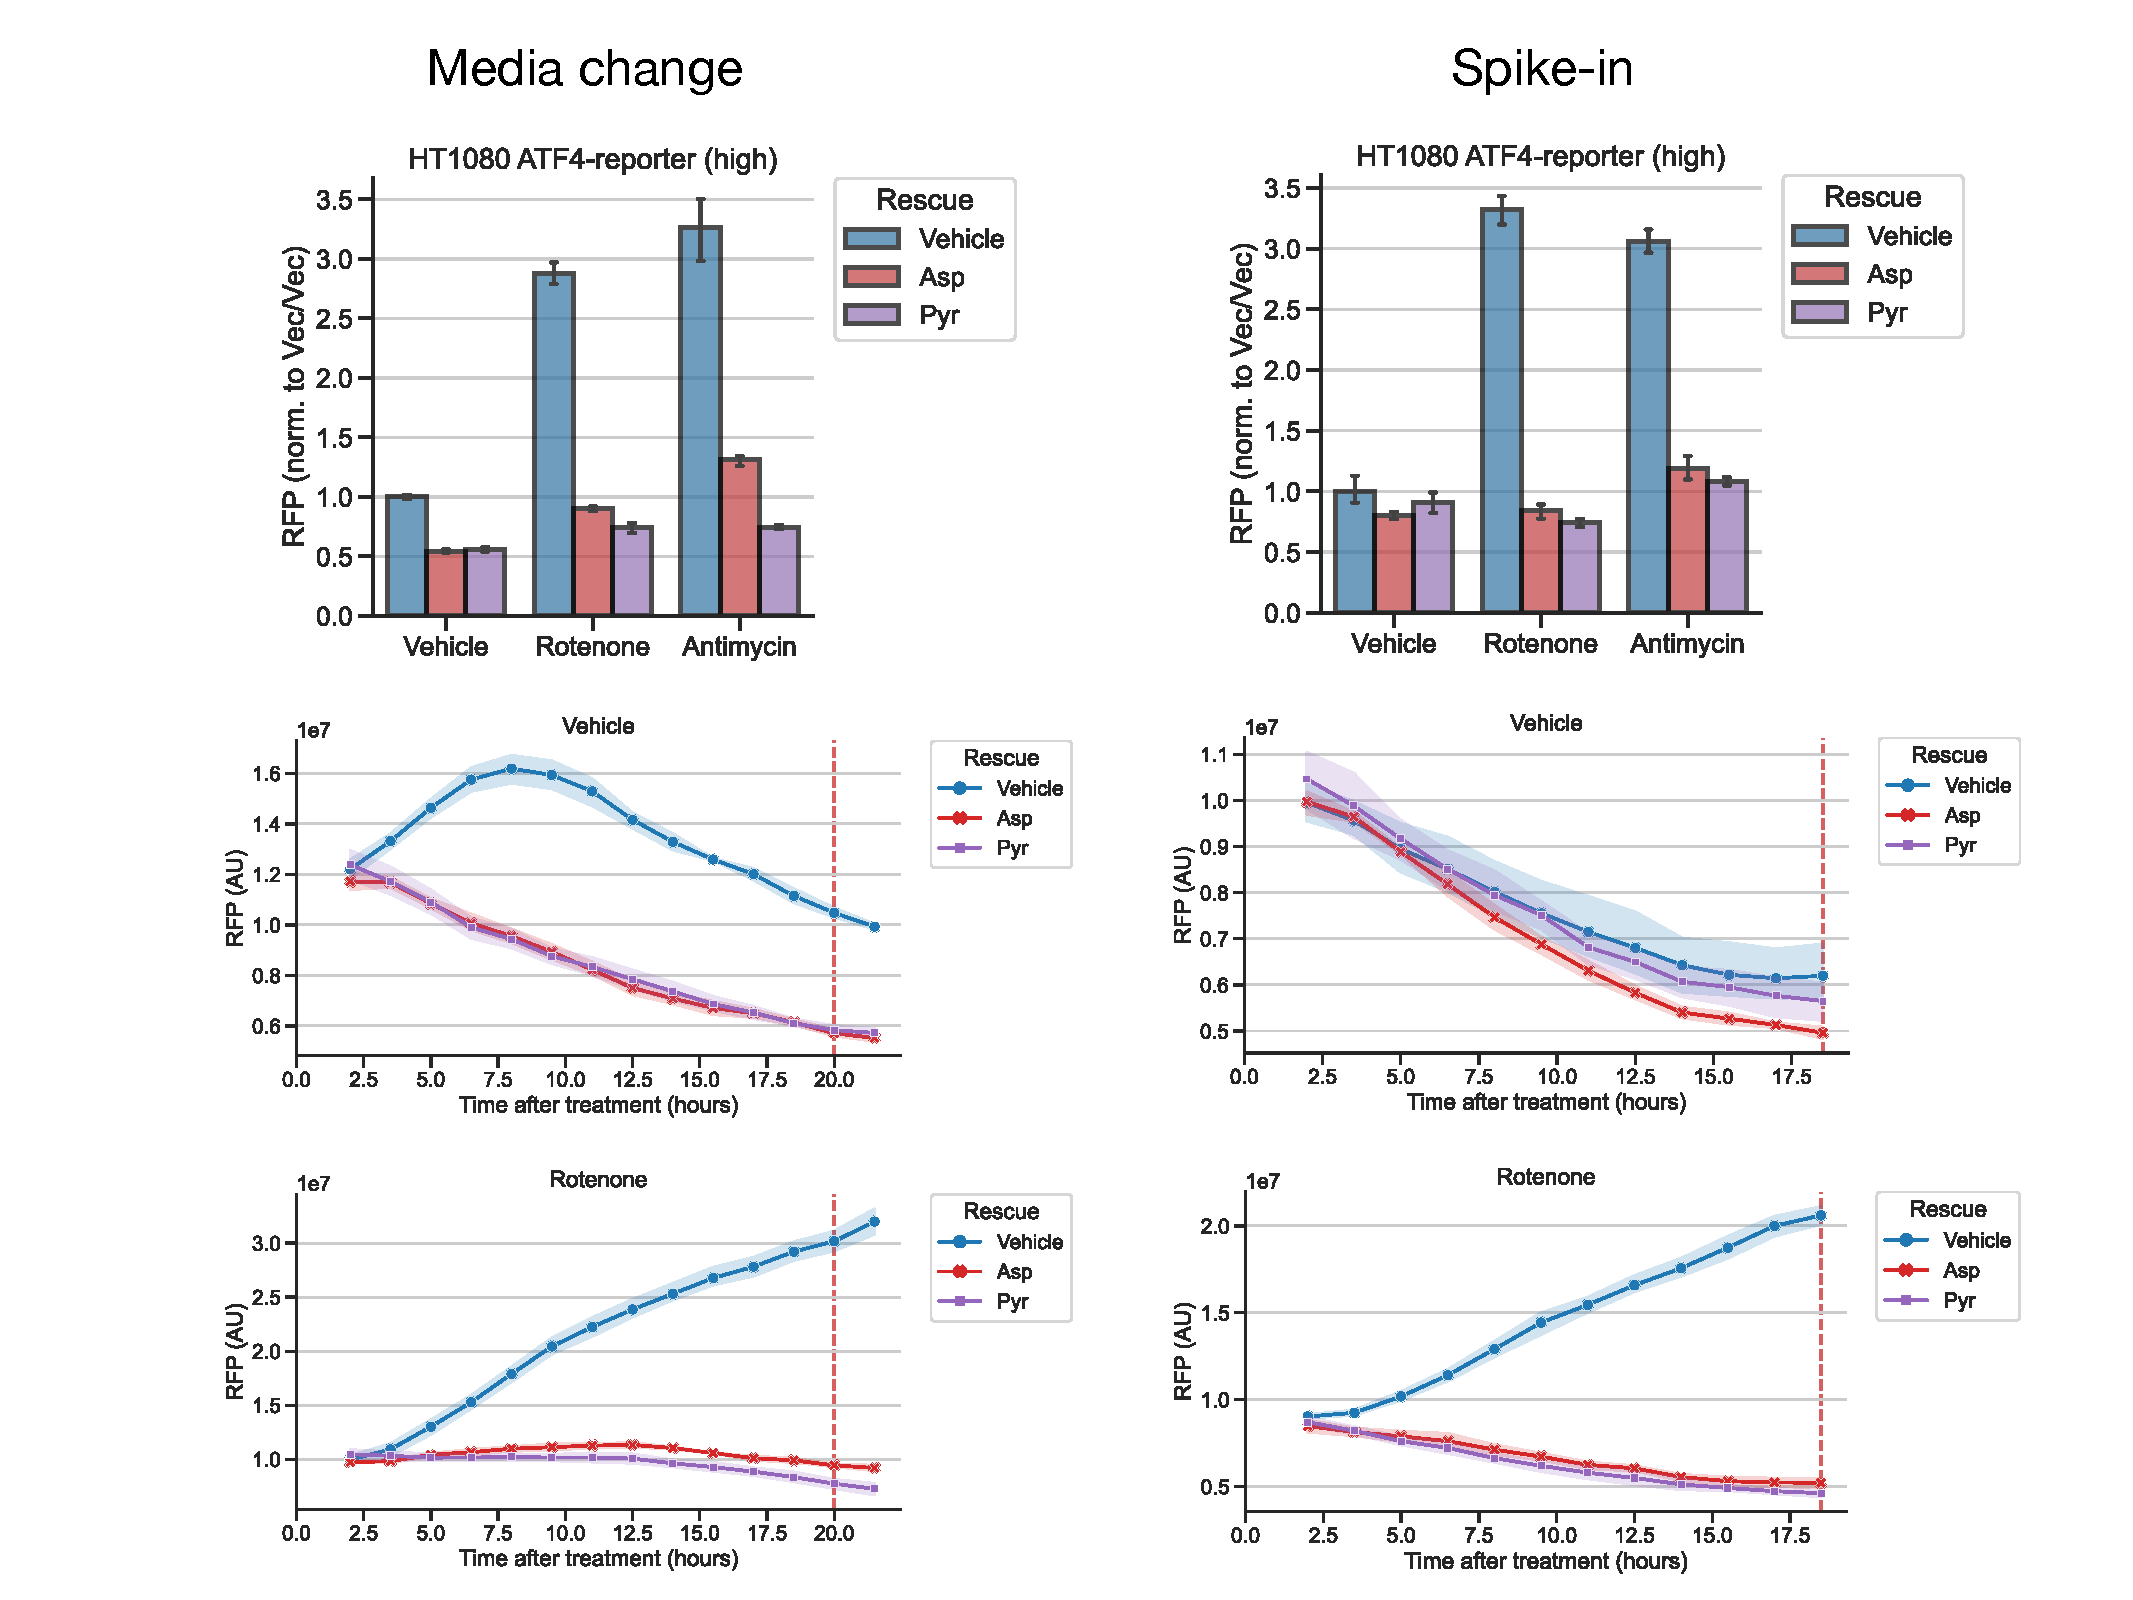
\includegraphics[width=0.95\textwidth]{figures/chap2/app/atf4_chVSsp.pdf}
    \caption[APP GGGG]{
    gggg
    }
    \label{fig:app_ch2:sal_frac_conc}
\end{figure}


\begin{figure}
    \centering
    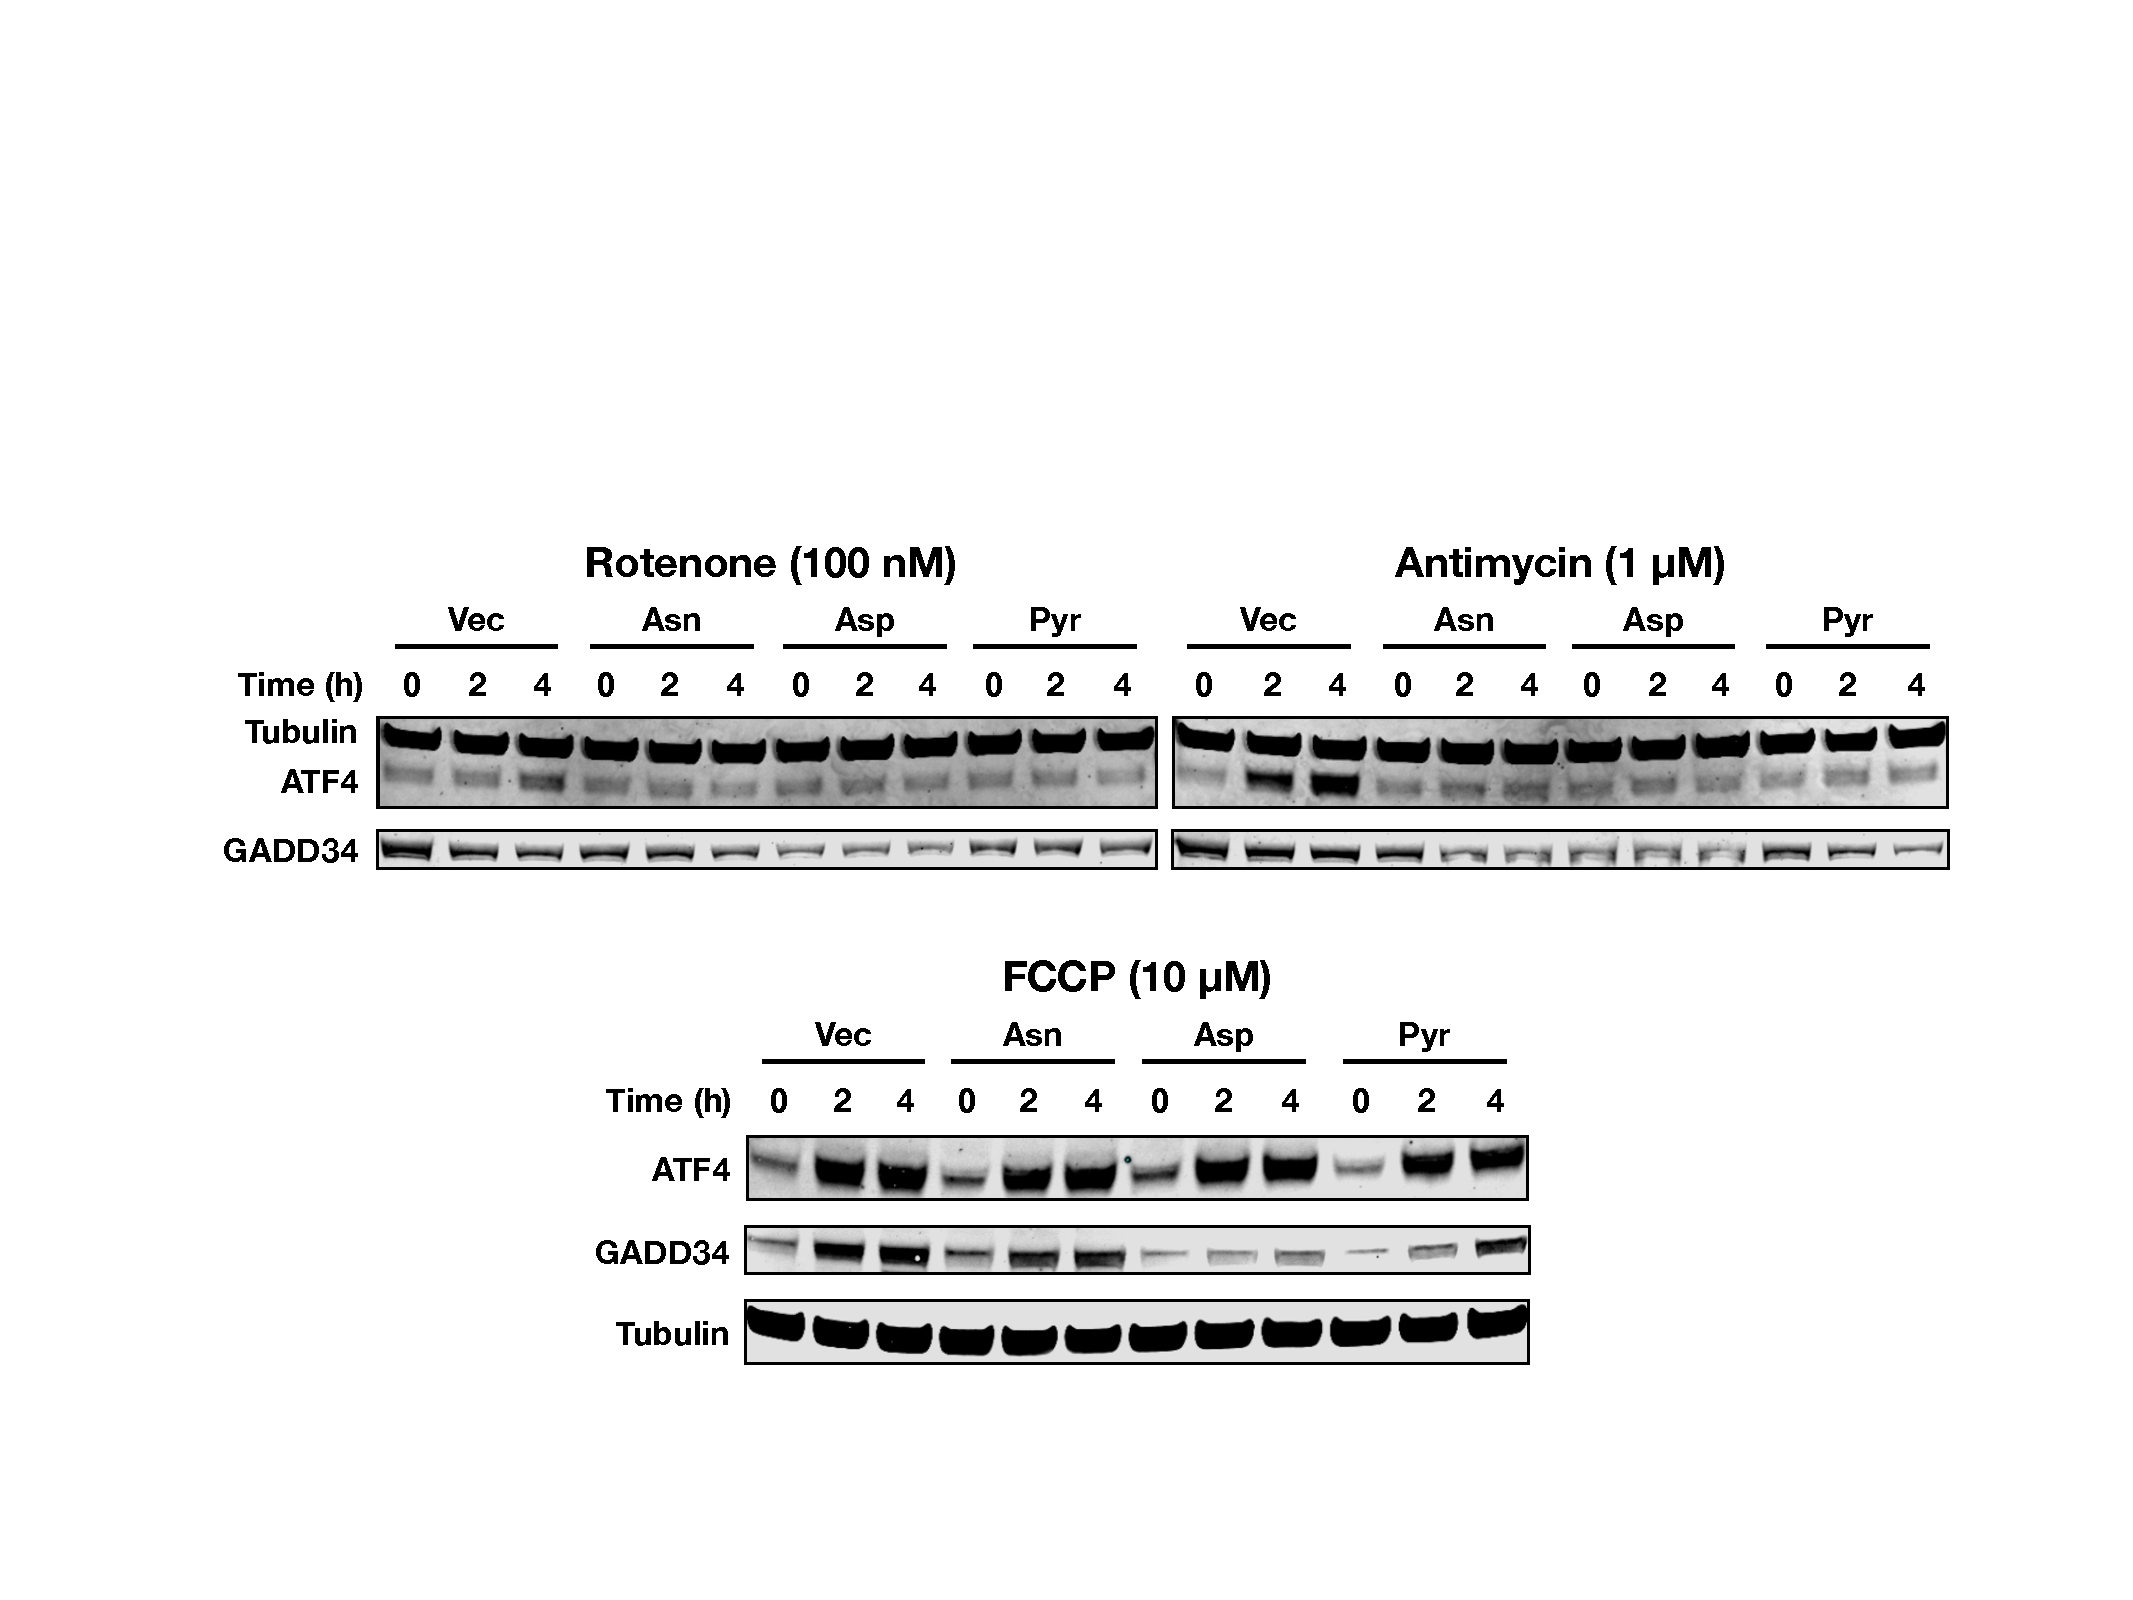
\includegraphics[width=0.95\textwidth]{figures/chap2/app/HT1080_ISR_western.pdf}
    \caption[APP GGGG]{
    gggg
    }
    \label{fig:app_ch2:HT1080_ISR_western}
\end{figure}



\begin{figure}
    \centering
    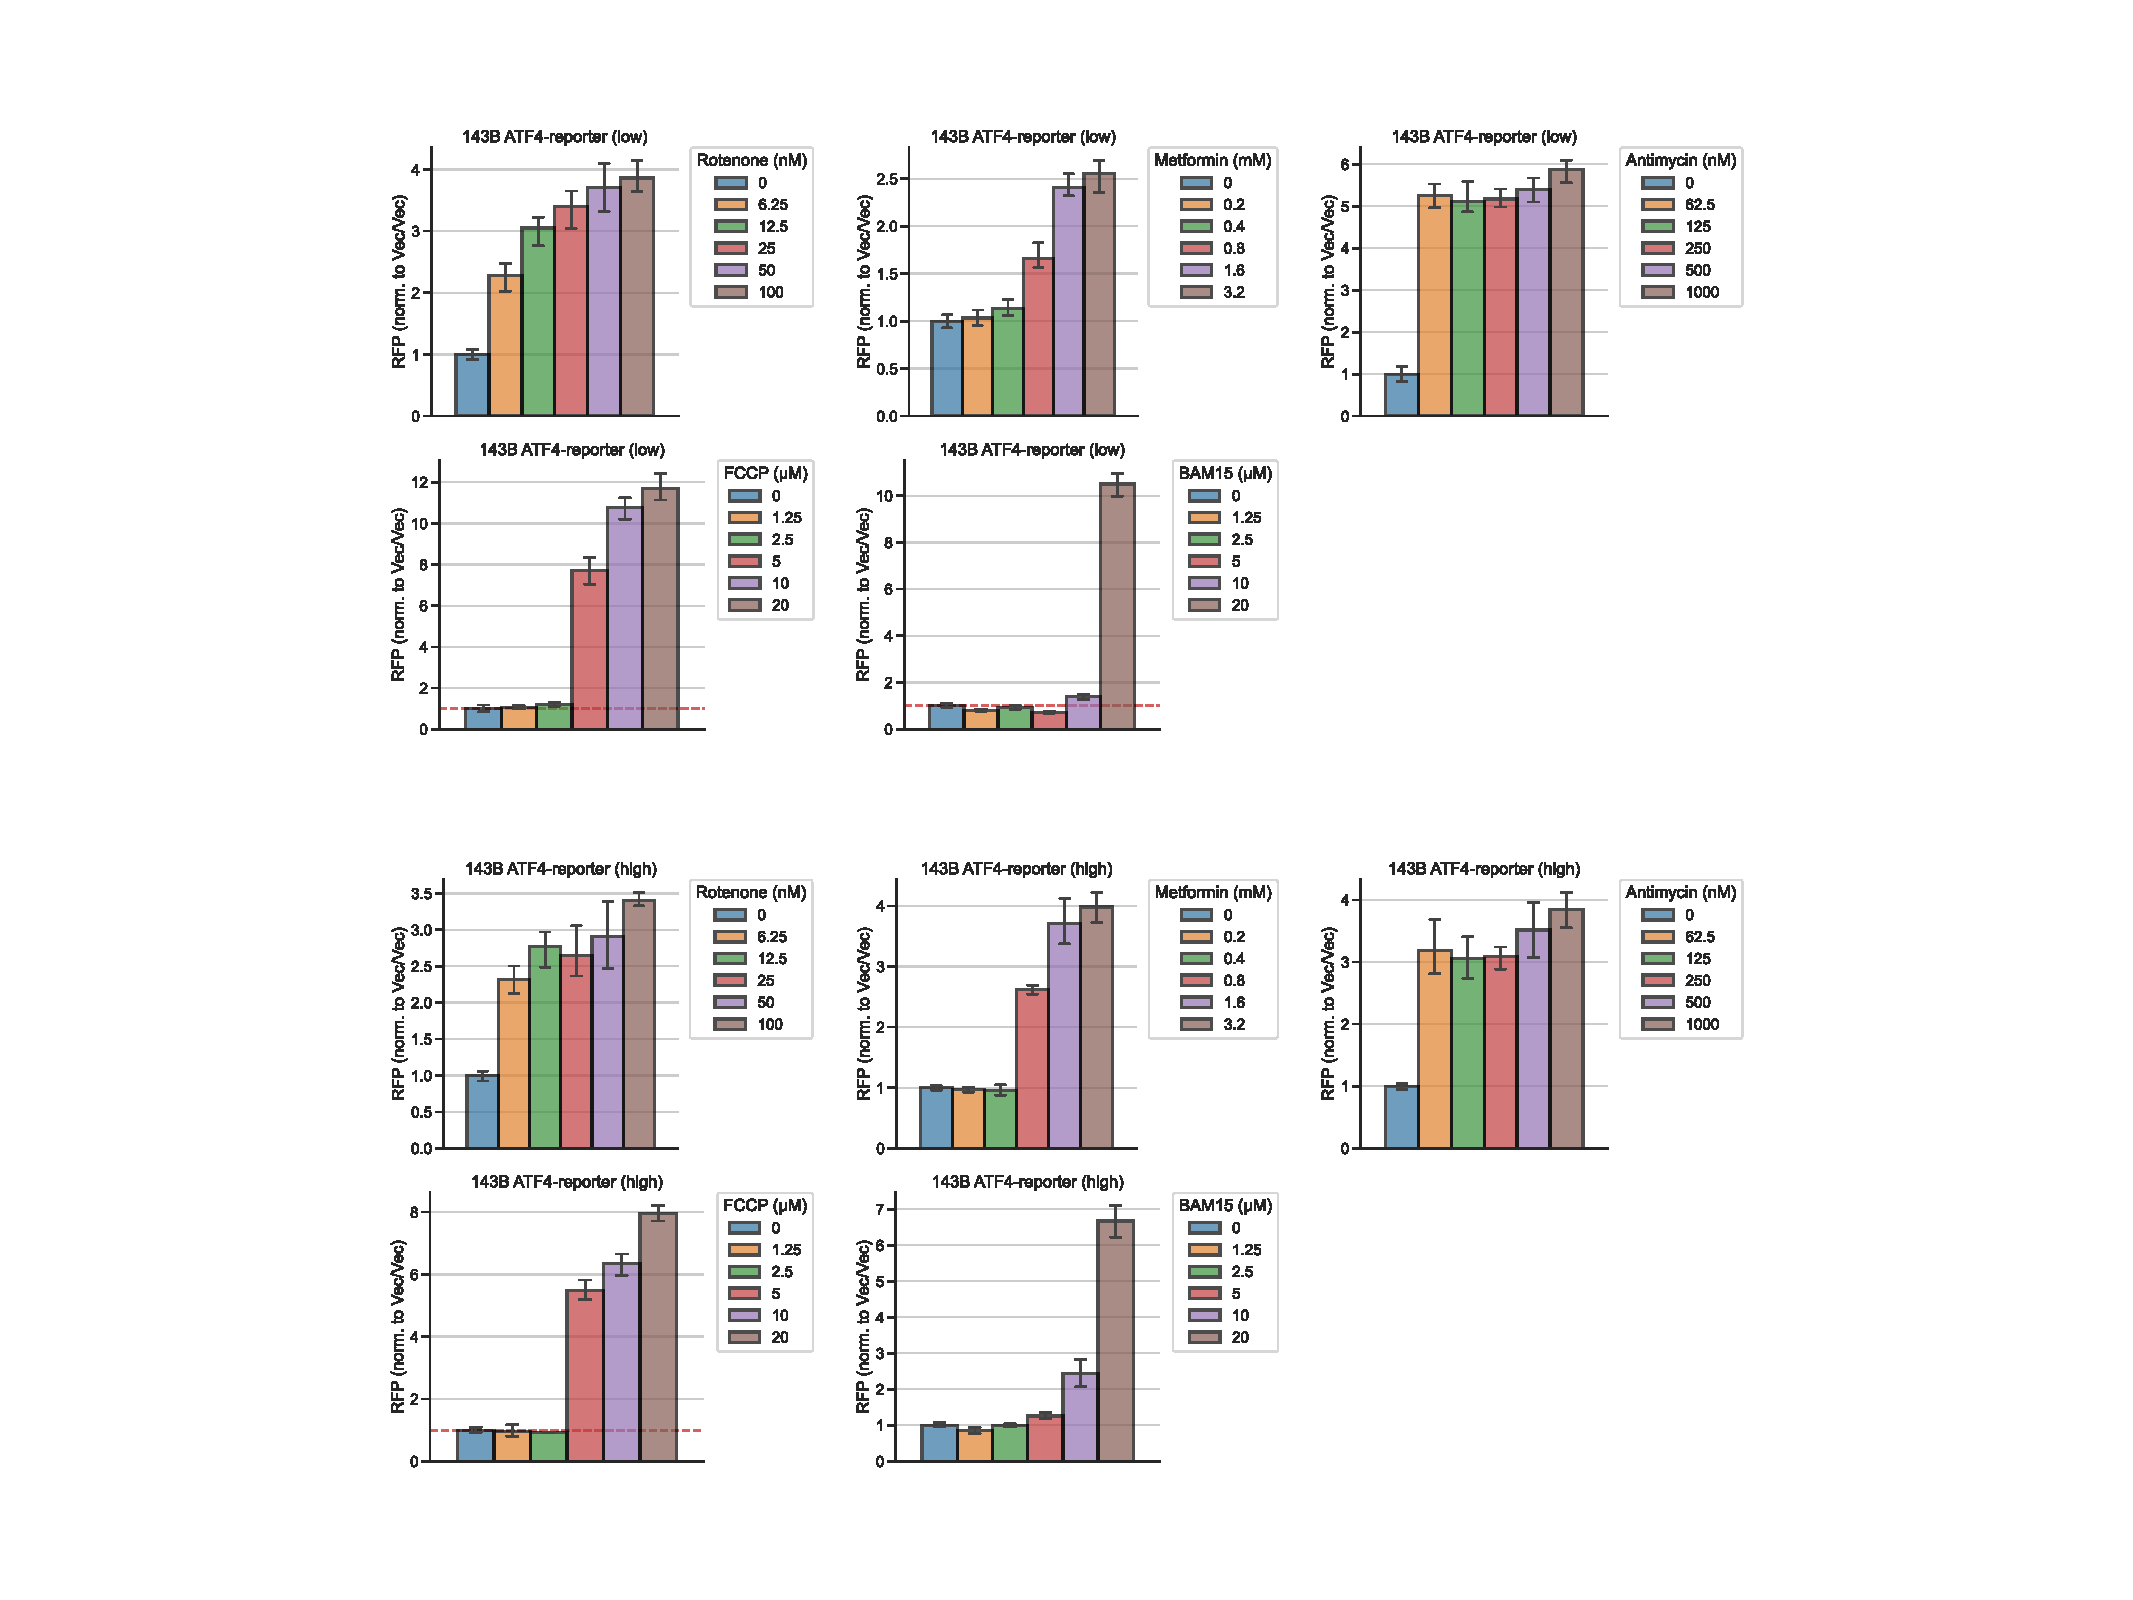
\includegraphics[width=0.95\textwidth]{figures/chap2/app/atf4_ETCtit.pdf}
    \caption[APP GGGG]{
    gggg
    }
    \label{fig:app_ch2:atf4_ETCtit}
\end{figure}




\begin{figure}
     \centering
     \begin{subfigure}[b]{0.49\textwidth}
         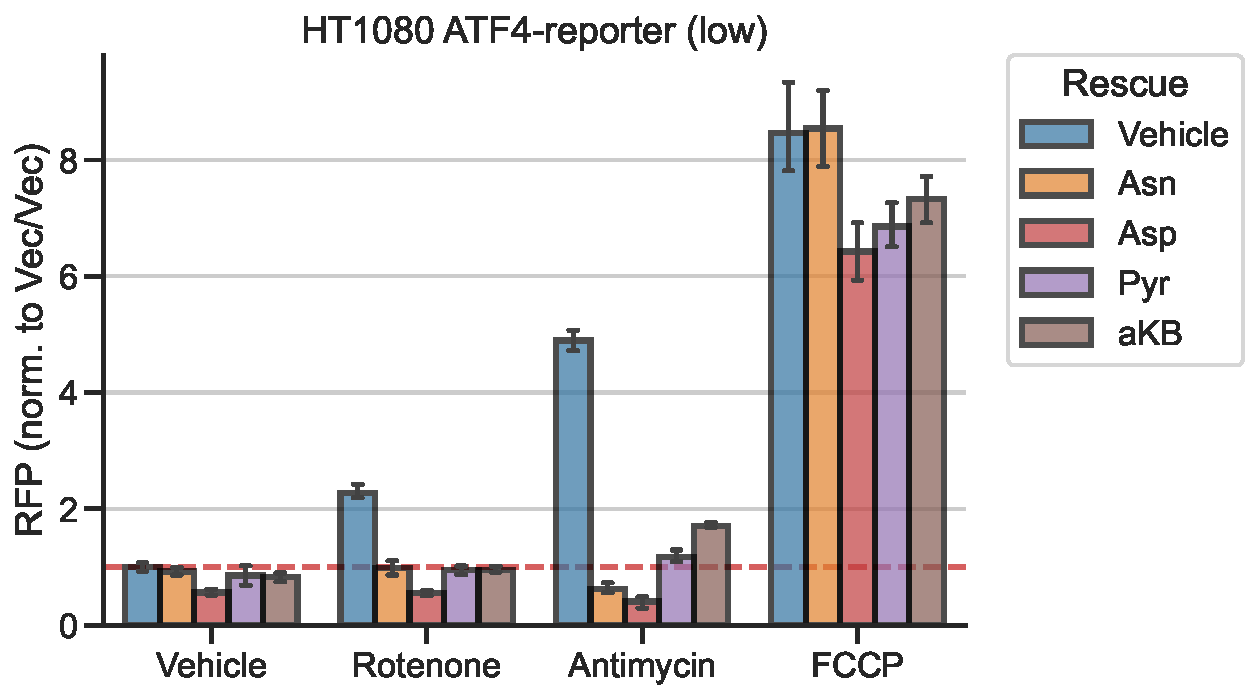
\includegraphics[width=\textwidth]{figures/chap2/app/HT1080_ETCinhib_ATF4rep_low.pdf}
         \caption{ggg}
         \label{fig:app_ch2:HT1080_ETCinhib_ATF4rep_low}
     \end{subfigure}
     \hfill
     \begin{subfigure}[b]{0.49\textwidth}
         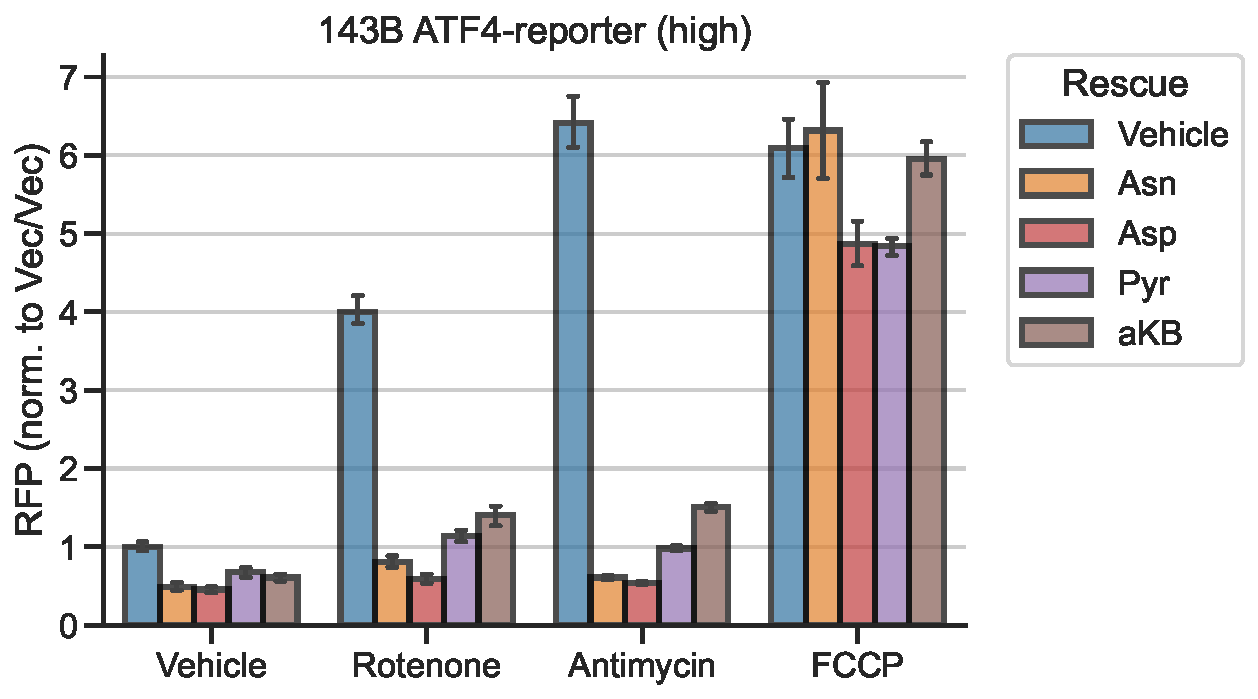
\includegraphics[width=\textwidth]{figures/chap2/app/143B_ETCinhib_ATF4rep_high.pdf}
         \caption{ggg}
         \label{fig:app_ch2:143B_ETCinhib_ATF4rep_high}
     \end{subfigure}
     \hfill
     \begin{subfigure}[b]{0.4\textwidth}
         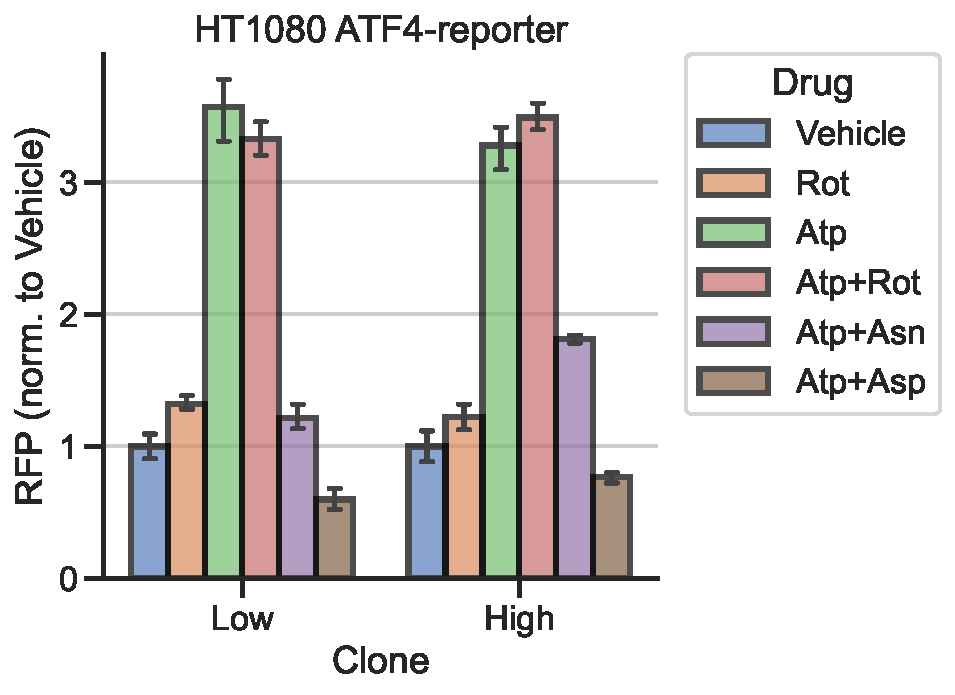
\includegraphics[width=\textwidth]{figures/chap2/app/HT1080_Atp_ATF4rep.pdf}
         \caption{ggg}
         \label{fig:app_ch2:HT1080_Atp_ATF4rep}
     \end{subfigure}
        \caption[ggg]{
        gggg
        }
        \label{fig:app_ch2:ISR}
\end{figure}











